\documentclass[]{sigplanconf}
\usepackage{stmaryrd}
\usepackage{listings}
\usepackage{multirow}
\usepackage{array}
\usepackage{subfig}
%\usepackage{algorithmic}
\usepackage{algorithm}
\usepackage{algpseudocode}
\usepackage{amsmath}
\usepackage{xfrac}
%\usepackage{amsthm}
\usepackage{amssymb}
\usepackage{xspace}
%\usepackage[pdftex]{graphicx}
\usepackage{graphicx}
\usepackage{siunitx}
\usepackage[svgnames,table]{xcolor}
\usepackage{natbib}
\usepackage{adjustbox}
\usepackage{tabularx}
\usepackage{booktabs}
\usepackage{placeins}
\usepackage{hyperref}
\usepackage{tikz}
\usetikzlibrary{automata,positioning}
%\usepackage{amsmath,amsfonts,amssymb,mathtools,url,cite,xspace,graphicx,color,stmaryrd,multirow,verbatim,listings,tikz,pspicture,epstopdf,algorithm,listings,algorithmicx,algorithm,caption,todonotes,algpseudocode}
\hypersetup{
    colorlinks,
	linkcolor={blue!50!black},
	citecolor={blue!50!black},
	urlcolor={blue!80!black}
}
\urlstyle{same}

%\newcommand\comment[1]{\ding{110}\ding{43}\textcolor{red}{#1}}

%\newcommand\code[1]{\textsf{\small #1}}
%\DeclareCaptionType{copyrightbox}
\newcommand\sius[1]{\num[group-separator = {,}]{#1}\si{\micro\second}}
\newcommand\sims[1]{\num[group-separator = {,}]{#1}\si{\milli\second}}
\newcommand\sins[1]{\num[group-separator = {,}]{#1}\si{\nano\second}}
\newcommand\tuple[1]{\langle #1 \rangle}
\providecommand{\abs}[1]{\lvert#1\rvert}

%\newcommand{\mc}[3]{\multicolumn{#1}{#2}{#3}}

\begin{document}

\title{Mining timed regular expressions from system traces}

\authorinfo{Greta Cutulenco, Yogi Joshi, Apurva Narayan, and Sebastian Fischmeister}
		   {University of Waterloo, ON, Canada}
		   {\{gcutulen, y2joshi, apurva.narayan, sfischme\}@uwaterloo.ca}

\maketitle


\begin{abstract}

Dynamic behavior of a program can be assessed through an examination of events emitted by the program during execution. For the behavior to be correct it must satisfy a set of specified temporal properties. Temporal properties define the order of occurrence and timing constraints on event occurrence. Such specifications are important for safety-critical real-time systems for which a delayed response to an emitted event may lead to a fault in the system. Since temporal properties are rarely specified for programs and due to the complexity of the formalisms, temporal properties are automatically extracted from traces of program execution. We propose a framework for automatically mining properties that are in the form of timed regular expressions (TREs) from system traces. Using an abstract structure of the property the framework constructs a finite state machine (FSM) to serve as an acceptor. We evaluate our technique on real-world datasets. We formally demonstrate the scalability and performance of our approach by running our implementations on synthesized traces of different sizes with different parameter values.

\end{abstract}

\section{Introduction}
%% author: AN
Temporal behavior of programs has been extensively studied~\cite{lamport1978time, dwyer1999patterns}. Recently, the idea of mining system traces to derive likely temporal specifications of programs has become popular~\cite{lemieux2015general}. Mining techniques generally identify a set of specifications which are satisfied by traces w.r.t. certain criteria. Commonly used patterns of specifications are provided for mining a systems' specifications. Many programs lack formal temporal specifications, and mined specifications are therefore valuable and could be used for a wide variety of activities in software development life cycle (SDLC). These activities include software testing~\cite{dallmeier2010generating}, automated program verification~\cite{kincaid2015automated}, anomaly detection~\cite{christodorescu2008mining}, debugging~\cite{gabel2010online}, etc. Further, mined specifications can assist automated verification techniques because they provide an easy and user-friendly way to describe programs' specifications. As argued by Ammons et al.~\cite{DBLP:conf/popl/AmmonsBL02}, automated verification techniques are unlikely to be widely adopted unless cheaper and easier ways of formulating specifications are developed. Consequently, specification mining has gained significant attention in recent times. Different techniques have been developed for mining specifications using templates expressed using regular expressions, LTL and other custom formats.

Most of the existing research in the context of mining temporal specifications focuses on qualitative notion of time, i.e., the specifications describe an \emph{ordering} of events. For example, an LTL specification $\Box(\mathrm{request}\,\rightarrow\,\lozenge \mathrm{response})$ specifies that a \emph{request} event should always be eventually followed by a \emph{response} event. Most state-of-the-art techniques do not take into account a \emph{quantitative} notion of time, i.e., the actual duration of time between events is not considered. For safety-critical real-time systems, it is important to develop techniques, which allow mining of specifications that account for the quantitative notion of time. For example, mining specifications of interrupt handlers, which complete their executions within a set of predefined deadlines for a real-time system, involves consideration about the quantitative notion of time. Such specifications are of important for safety-critical real-time systems for which a delayed response to an emitted event may lead to a fault in the system. Certain specifications of real-time systems can be modeled using timed regular expressions, which can be in turn translated into the corresponding timed automata.

With a motivation to address the problem of mining specifications with explicit notion of time, we propose a technique to mine instances of timed regular expression (TRE)~\cite{timedregex} templates satisfied by a given system's traces. TREs extend regular expressions by providing additional operators to specify timing constraints between events. By using a set of commonly used patterns of specifications for LTL and regular expressions, we develop the corresponding patterns for TREs. Further, we use the method proposed by Asarin et al. \cite{timedregex} to synthesize the timed automaton for a given TRE. Such timed automaton is then used as a checker to verify whether traces satisfy the corresponding TRE. TRE templates replace actual events in a TRE instance by a variable, which can be assigned a value of an actual event in traces. We provide two algorithms for mining instances of TREs from their templates. Both algorithms require a TRE template and a system's traces as input. The algorithms then use the distinct events in the traces to generate different possible \emph{permutations} of the events that can be formed by substituting the actual events into the variables in the TRE template. Intuitively, the given trace is processed against every permutation to check whether the trace satisfies TRE instances denoted by the corresponding permutations. Further, we define \emph{support} and \emph{confidence} as metrics to evaluate the degree to which a TRE instance is satisfied by a trace. The algorithms then report the permutations which satisfy the given threshold values of support and confidence.

The first algorithm is designed for TRE templates containing negation operator. The second algorithm processes TRE templates without a negation operator. We later prove that although both algorithms' execution times are exponential in terms of the number of variables in individual TRE templates, the second algorithm generally runs faster than the first by a certain factor which depends upon the number of distinct events in a trace and the number of variables in a given TRE template. We also prove that our technique is sound, i.e., a mined specification reported by our algorithms actually satisfies the given thresholds of support and confidence on the provided input traces. Also, our technique is complete, i.e., our algorithms report all TRE instances which comply on given traces w.r.t. the thresholds of support and confidence.

We evaluate our technique on real-world datasets which consist of logs produced by QNX realtime RTOS  \cite{QNX_RTOS} during various runs of application software on different hardware platforms and controller area network (CAN) \cite{CAN}traces of an automobile. We report the performance of our algorithms in terms of the execution time. We demonstrate the scalability and performance of our approach by running our implementations on synthesized traces of different sizes with different values of parameters such as the number of distinct events, the total number of events in traces and the complexity of TRE templates.

In this paper we propose a framework to automatically mine properties that are in the form of timed regular expressions from system traces. Using an abstract structure of the property the framework constructs a finite state machine (FSM) to serve as an acceptor. We encode the concrete properties in a set of matrices. The FSM is used to evaluate the satisfaction of every potential concrete property in the trace. Using a ranking system we infer the strongest concrete properties that describe the system and thus deduce a set of interesting system specifications.

The key contributions of this paper involve developing an efficient framework for extracting complex temporal properties that take on the form of timed regular expressions and evaluating the framework experimentally on industrial real-time systems:

\begin{itemize}
\item We develop two novel algorithms to mine instances of timed regular expressions satisfied by a given system's traces. To our knowledge, this is the first technique for mining specifications with explicit notion of timing constraints (Section ~\ref{Approach}),
\item Identifying computational approaches that optimize the extraction of the specified properties (Section ~\ref{Approach}),
\item Demonstrating the frameworks' applicability to large traces collected from real industrial systems  (Section ~\ref{discussion}).
\end{itemize}


%% author: GC

%Dynamic behavior of a program can be assessed through an examination of events emitted by the program during execution. For the behavior to be correct it must satisfy a set of specified temporal properties. Temporal properties constrain the order of occurrence of the emitted events. Temporal properties also impose timing constraints on event occurrence. Such specifications are of importance for safety-critical real-time systems for which a delayed response to an emitted event may lead to a fault in the system.

%Since temporal properties are rarely specified for programs and due to the complexity of the formalisms, temporal properties are automatically extracted from traces of program execution. Dynamic specification inference has shown promising results in many areas, including bug detection, test case specification, and program steering~\cite{evans2}. The properties can be used to ensure that the system does only what is specified and nothing else. They can be used to evaluate testing completeness - all specified properties are exhibited through existing tests. And lastly they can be used to compile a detailed and complete set of system specifications.

%The currently available approaches for extracting temporal properties are however insufficient \cite{abc}. They do not scale well for interesting properties with a large number of events. They cannot extract properties efficiently from large and complex system traces and do not support extraction of properties with timing constraints.




\section{Background} \label{Background}

\subsection{Timed Regular Expressions}

Classical automata theory handles only the \emph{qualitative} notion of time, i.e. a sequence of events specifies the ordering of events but not the time between the occurrence of these event in terms of ``real time". An abstraction of this sort has been found useful for analysis of certain systems, whereas many application domains require more detailed models which include accurate timing information. For example, we might want to modify a formal specification from ``a is followed by b" into a more precise specification with timing information as `` a is followed by b within $x$ seconds". We need to develop algorithms for mining specification with timing information. Timed automata \cite{AD94} (automata equipped with clock) has been investigated quite rigourously in the recent past. The main motivation of using timed automata is due to their suitability for modeling time-dependent behavior, and their ability to monitor their reachability \cite{LPY97}.

We will formally describe our nomenclature.

\newtheorem{defns}{Definition}

\begin{defns}[Trace and event]
The alphabets of events is a finite alphabet of strings. An ordered sequence of events is a trace.
\end{defns}

We use the term \emph{event} to denote a place holder for an event. We use Time Regular Expressions (TRE) \cite{timedregex} to provide specification templates.

\begin{defns}[Timed Regular Expression (TRE)\cite{timedregex}] Timed regular expressions over an alphabet $\Sigma$ (also referred to as $\Sigma$-expressions) are defined using the following families of rules.
\begin{itemize}
  \item  \underbar{a} for every letter a $\in \Sigma$ and the special symbol $\epsilon$ are expressions
  \item If $\phi$, $\phi_1$ and $\phi_2$ are $\Sigma$ expressions and $I$ is an integer bound interval then $\langle \phi \rangle_I$, $\phi_1 \dot \phi_2$, $\phi_1 \vee \phi_2$ and $\phi^*$ are $\Sigma$ expressions.
\end{itemize}
\end{defns}


\begin{defns}[TRE Templates] A TRE template is a TRE in which all of the atomic propositions are either event variables, events or time interval.
\end{defns}
For example, the TRE template $<0.1>[x,y]$ represents the ``0 is always followed by 1 within the time interval [x,y]'', where $x \le y$ and are fixed doubles.

A TRE instance corresponds to a TRE template and has an identical TRE structure. With each event variable in the TRE template when replaced by an event, we refer to the map as $binding$.

\begin{defns}[TRE Instance]
Let $\Pi$ be a TRE template. Then, $\pi$ is a TRE instance of $\Pi if \pi$ has a TRE similar to $\Pi$ in structure and where all the atomic propositions are events.
\end{defns}

\begin{defns}[Binding]
Let $\Sigma$ be an alphabet of events and let $V$ be a finite set of event variables. Then, a binding is a function $b \colon V \rightarrow \Sigma$
\end{defns}

Applying a binding to the variables in a TRE template creates a TRE instance corresponding to that binding. We express that a binding and its corresponding TRE instance are valid on a trace if the TRE instance holds on each trace in the log. Generally, we are interested in mining all of the valid TRE instances.

\begin{defns}[Trace Support Potential]
Trace support potential of a TRE instance $\pi$ on a trace $t$ is the number of time points of $t$ which could falsify $\pi$.
\end{defns}

\begin{defns}[Trace Confidence (To be Verified)]
Trace Confidence of a TRE $\pi$ on a trace $t$ is the number of time points of $t$ which could falsify $\pi$ but do not falsify $\pi$.
\end{defns}

As we propose a framework that mines properties in the form of TREs from system traces using an abstract structure of the property using a finite state machine (FSM) to serve as an acceptor. We use the formalism of Timed automata for our purpose as it allows for enforcing explicit timing constraints in the model.

\subsection{Timed Automata}

Timed automata is a theory for modeling and verification of real time systems.  Explicit timing constraint are naturally present in real-life systems. Classical models (finite automata, Petri-nets etc.) cannot express such real time constraints. Time automata \cite{Alur1990, Alur1994183} has been used extensively for modeling real-time systems. One of the most important properties of the timed automata is probably that the reachability properties are decidable \cite{Alur1994183} even though the timed automata have infinite number of configurations. The main idea behind this result is the construction of region-automaton, which finitely abstracts the behavior of timed automata in a way that checking reachability in a timed automata reduces to checking reachability in a finite automaton.

\begin{defns}[Timed Automata \cite{timedregex}]
A timed automaton  $\mathcal{A}$ is a tuple $\langle Q,C,\Delta ,\Sigma, s,F\rangle$ where $Q$ is a finite set of states, $C$ is a finite set of clocks, $\Sigma$ is an input (or event) alphabet, $\Delta$ is a transition relation, $s \in Q$ an initial state and $F \subset Q$ a set of accepting states. The transition relation consists of tuples of the form $\langle q ,\phi ,\rho, a, q' \rangle$ where $q$ and $q'$  are states, $a \in \Sigma \cup \{\epsilon \}$ is a letter, $\rho \subseteq C$ and $\phi$ (the transition guard) is a boolean combination of formulae of the form $(x \in I)$ for some clock $x$ and some integer-bounded interval $I$.
\end{defns}

A clock valuation is a function $v \colon C \rightarrow \mathbb{R}^+$, or equivalently a $|C|$-dimensional vector over $\mathbb{R}^+$. We denote the set of all clock valuations by $\mathcal{H}$ . A configuration of the automaton is hence a pair $(q,v) \in Q \times H$ consisting of a discrete state (sometimes called “location”) and a clock valuation. Every subset $\rho \subseteq C$ induces a reset function $Reset_\rho : H \rightarrow H$ defined for every clock valuation $v$ and every clock variable $x \in C$ as

\begin{equation}\label{timed_automaton}
Reset_\rho v(x) = \begin{cases}
0, & \text{if $x \in \rho$} \\
v(x) &\text{if $x \notin \rho$}
\end{cases}
\end{equation}

$Reset_\rho$ resets all the clocks in $\rho$ to zero and leaves the other clocks unchanged.

\begin{figure}
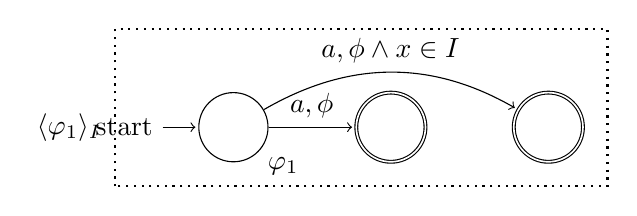
\begin{tikzpicture}[shorten >=1pt,node distance=2cm,on grid,auto]
   \draw[very thick,black](-1.5,0) node[left=1pt,fill=white]{$\langle \varphi_1  \rangle_I$};
   \draw[very thick,black](1,-0.5) node[left=1pt,fill=white]{$\varphi_1$};
   \node[state, initial] (s) {};
   \node[state, accepting] (f) [right=of s] {};
   \node[state, accepting] (f1) [right=of f] {};
   \path[->]
    (s) edge node {$a, \phi$} (f)
        edge [bend left] node {$a,\phi \wedge x\in I$}(f1);
    \draw[thick,dotted] (-1.5,-0.75) rectangle (4.75,1.25);
\end{tikzpicture}
\caption{Timed Automata from a Timed Regular Expression}
\label{fig:tretoautomata}
\end{figure}

It has been proved \cite{timedregex} that every timed regular language can be recognized by a timed automaton.  We present a simple example of representing the TRE using timed automata and vice-versa. The basic idea behind construction of a timed automata $\varphi^*$ is that we need the values of all the clocks at each new iteration of $\varphi$ to represent the total time elapsed in the previous iterations. This is achieved by adding a new clock $x$ which is never reset to zero and transitions to the initial state in which all the clocks get the value of $x$. In Figure \ref{fig:tretoautomata} we see that a new clock $x$ and a test $x \in I$ has been added to guard every transition leading to final state.

The novel features here with respect to untimed regular expressions are the meaning of the atom $\underline{\alpha}$ which represents an arbitrary passage of time followed by an event $\alpha$ and the $\textless \Phi \textgreater _I$ operator which restricts the metric length of the time-event sequences in [[$\Phi$]] to be in the interval I.

The '.' is the concatenation operator and the '+' is the operator for one or more instances of the expression.

\section{Approach} \label{Approach}
%% author: GC

\begin{figure}[h]
  \centering
  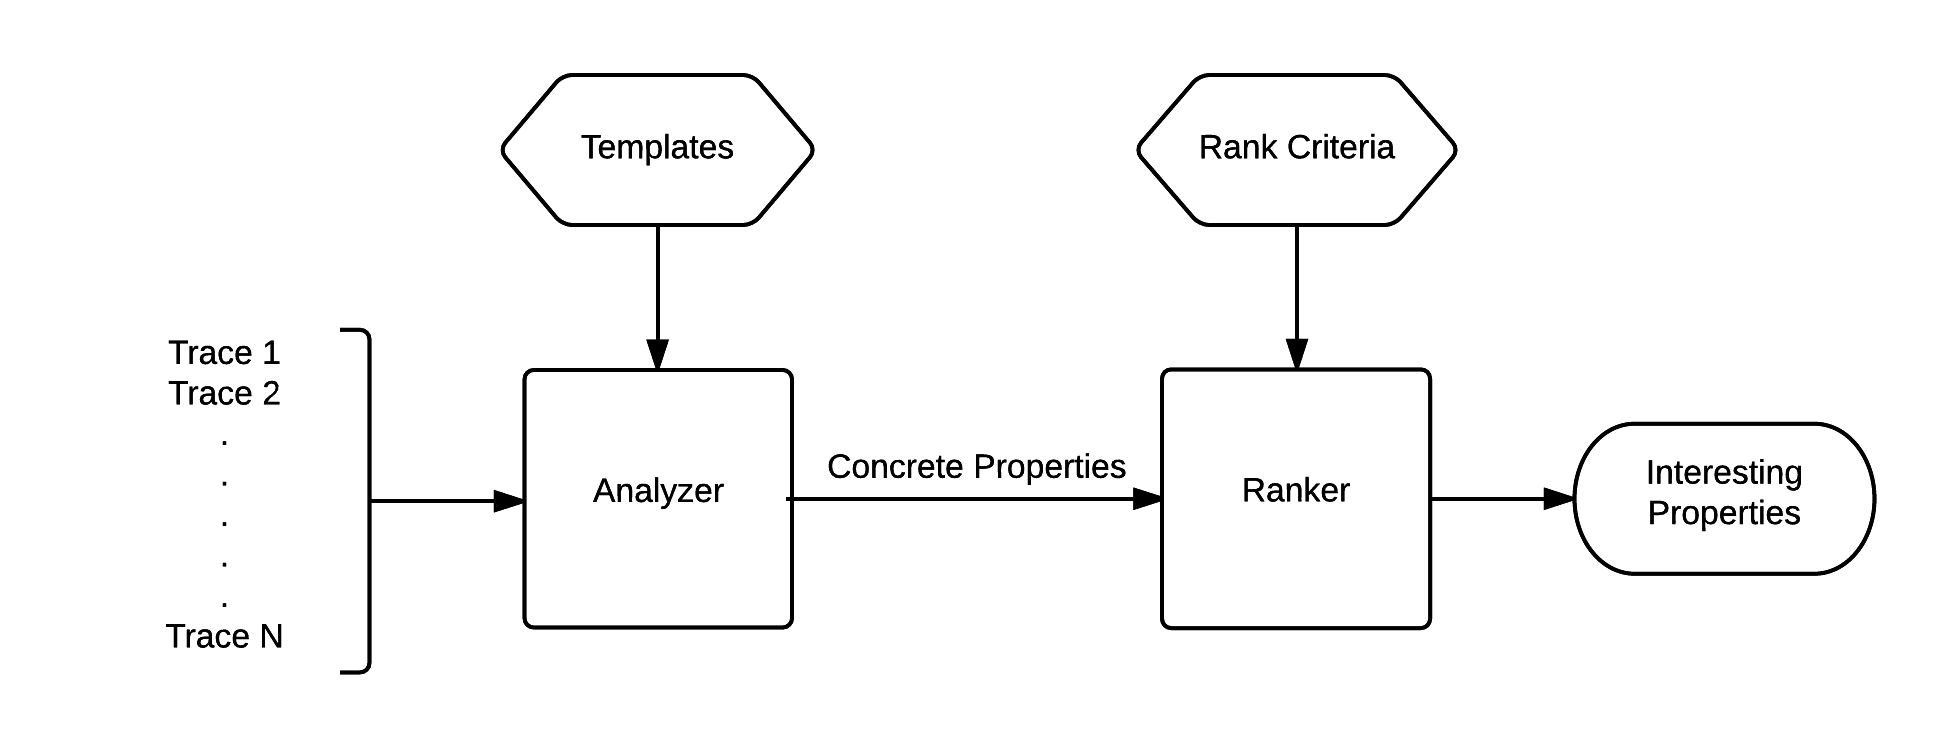
\includegraphics[trim = 1cm 0cm 0cm 0cm,clip = true,width=\linewidth]{figures/Workflow.png}
  \caption{Property Mining Workflow}
  \label{fig:work-flow Overview}
\end{figure}

\subsection{The Workflow} \label{the_workflow}

We use traces of execution collected during the runtime of a system. The event traces are generated using instrumentation already present in the system and include network traffic logs, operating system logs, or program instrumentation logs. The analyzer accepts a set of N logs, where N $\ge$ 1.

The templates in ~\ref{fig:work-flow Overview} refer to templates of temporal properties - timed regular expressions ~\cite{timedregex} that encode constraints on the relationships between subsets of trace events. Each template is an abstraction of the desired temporal property, like request, alternating, etc. ~\cite{evans1}. A template uses an abstract set of symbols ranging from 0 to L, where L is the length of the abstract alphabet. It also uses operators and time intervals as defined in ~\cite{timedregex}. For instance, (1.\textless0\textgreater[2,5])+ is a template for the response pattern. The '.' is the concatenation operator and the '+' is the operator for one or more instances of the expression.  The template specifies that some log event 1 is followed by another log event 0 within 2 to 5 time units, and this pattern occurs at least once in the execution trace.

The abstract alphabet is used as a placeholder. The analyzer extracts a set of S unique event symbols from the collected traces and substitutes these in place of the abstract symbols to form concrete temporal properties. In the case of (1.\textless0\textgreater[2,5])+ the analyzer will evaluate the property for all combinations of two events in S. The key insight for achieving O(nL) time complexity is that an event X from the trace can be treated as either a P event or an S event.

Using an incidence matrix of dimension L we will evaluate which event combinations satisfy the given property. The acceptor FSM will iterate over the events in the system log and at each new event evaluate if any of the combinations in the matrix are satisfied. The matrix keeps track of the number of successes and failures to evaluate each concrete temporal property.


An intuitive way to evaluate a time regular expression on a system execution trace is to over the trace and recursively evaluate the TRE according to its semantics. A high level description of our algorithm is presented in


\begin{itemize}
\item \textbf{Representing a TRE} We parse the input timed regular expression and transform it into a timed automata.
\item \textbf{Representing a trace} We parse the input trace into a  linear array representation where each unique event has its corresponding time and event id [time, eventid].
\item \textbf{Checking property instances over traces} We iterate over the set of each unique event and process the entire trace with respect to each unique event. Updating the \emph{success} and \emph{reset} for the entire trace. Processing the trace refers to matching the required TRE in the process trace.
\end{itemize}


\begin{algorithm}[h]
    \caption{Timed Regular Expression Mining}\label{alg:the_alg}
    \begin{algorithmic}[1]
     \Require  Given a set of traces with unique event \emph{i} and a TRE pattern
     \Ensure Parse TRE and formulate a finite Timed Automaton $\rightarrow$ A
     \State Initialize the incidence matrix of size $\Sigma^p$
     \State Initialize the \emph{success} and \emph{reset} counters for all permutations
     \For {(each unique event $i$ from the trace)}
        \State Process the complete trace;
        \State Update the success if A $\rightarrow$ FS;
        \State Update the reset if A $\rightarrow$ ES;
     \EndFor
     \State Evaluate Support - S
     \State Evaluate Confidence - C
    \end{algorithmic}
\end{algorithm}

In Algorithm ~\ref{alg:the_alg} $\Sigma$ is the set of alphabets and $p$ is the number of place holders in the TRE. $A$ denotes the timed automaton and $FS$ and $ES$ denote the final and error states of the timed automaton. $S$ and $C$ denote the \emph{support} and \emph{confidence} metrics of the TRE on the given trace.

We used the most commonly occurring temporal property patterns \cite{evans} by transforming them into Time Regular Temporal Property patterns. Let us assume we have several causing events $P$ to share one effect event $S$. The TRE property patterns are presented in Table ~\ref{TRE_Exp}.
\begin{table}[ht]
  \centering
  \begin{tabular}{|c|c|}
  \hline
  % after \\: \hline or \cline{col1-col2} \cline{col3-col4} ...
  \textbf{Name} & \textbf{TRE}  \\ \hline
  Response      & $[-P]^*;((P;[-S]^*;S \langle x,y \rangle);[-P]^*)^*$        \\ \hline
  Alternating   & $[-P,S]^*;(P;[-P,S]^*;S;[-P,S]^* \langle x,y \rangle)^*$       \\ \hline
  MultiEffect   &  $[-P,S]^*;(P;[-P,S]^*;S;[-P]^* \langle x,y \rangle)^*$     \\ \hline
  MutiCause     &  $[-P,S]^*;(P;[-S]^*;S;[-P,S]^* \langle x,y \rangle)^*$     \\ \hline
  EffectFirst   &  $[-P]^*;(P;[-P,S]^*;S;[-P,S]^* \langle x,y \rangle)^*$      \\ \hline
  CauseFirst    &  $[-P,S]^*;(P;[-S]^*;S;\langle x,y \rangle [-P]^*)^*$       \\ \hline
  OneCause      &  $[-P]^*;(P;[-P,S]^*;S;\langle x,y \rangle [-P]^*)^*$       \\ \hline
  OneEffect     &  $[-P]^*;(P;[-S]^*;S;[-P,S]^* \langle x,y \rangle)^*$       \\ \hline
\end{tabular}
\caption{TRE Property Patterns}\label{TRE_Exp}
\end{table}

\subsection{Dominant Properties}

The concrete properties examined by the analyzer contain every permutation of trace events within the template. These contain both interesting and frequently occurring patterns, as well as those that might have been found just a handful of times in the trace. Since the number of concrete properties could be very large, $S^L$, a ranking component is used to reduce the set to interesting properties only.

The effectiveness of selecting a meaningful subset of properties depends on picking a good set of criteria and associated satisfaction thresholds. The ranking criterion we use is a combination of support and probability. Support is the percentage of all traces that contain the concrete property. Probability is the ration of successful evaluations of the property over total possible occurrences. We specify a threshold for these measures to extract properties that are consistently dominant in the collected traces. In section X our experiments explore the appropriate values for the thresholds.

Another motivation for using the ranker is the presence of imperfect traces. Traces can be imperfect as a result of dropped events or execution of faulty programs. In such cases, properties may not be perfectly satisfied in the collected traces. By using the probability and support ranking criteria we focus on finding the dominant properties in the trace.


\section{Discussion} \label{discussion}
%% author: GC

Our work mines temporal properties that can be expressed using timed regular expressions. The following discussion explores how the chosen approach accomplishes this and why it does so optimally.

\subsection{Using Timed Automata as Acceptors}

First we can look at regular expressions and their acceptors without the timing constraints. Regular expressions offer a declarative way to express the patterns that we want to accept. Every language defined by a regular expression is also defined by a finite automaton, as defined by Theorem 3.7 in ~\cite{book1}. There is a way to convert any regular expression into a non-deterministic automaton, and further to convert from a non-deterministic to a deterministic automaton. We can thus generate a Deterministic Finite Automaton (DFA) for any regular expression.

Similarly, timed automata are recognizers of timed languages. They have states, as any FSM, as well as clocks. Every timed language defined by a (generalized extended) regular expression is accepted by a timed automaton, as defined by Theorem 2 in ~\cite{timedregex}. Thus, timed automata and generalized timed regular expressions have the same expressive power.

The language of a timed automaton consists of all the strings that it accepts ~\cite{timedregex}. The strings in our case are sequences of time-event pairs. The timed automata we generate are acceptors for strings that satisfy the desired property. The more strings in the trace that can be accepted, the more dominant is the property.

\subsection{Memory Requirements}

The main space requirement of our approach is for containing the matrix. The dimensionality L of the matrix depends on the number of abstract symbols in the desired property. The more events present in the relationship that the property encodes, the more dimensions of the matrix will be required.

Each dimension of the matrix will consist of S unique event symbols. We want to encode the matrix to hold the evaluation results of every combinatorial combination of unique events. Thus we need $S^L$ space to hold acceptor results.

The number of unique events S in the trace will depend on the complexity of the program or system. However more concerning is the dimensionality since it will lead to exponential growth of the space requirements.

Majority of properties that people care about most represent relationships among a few events ~\cite{evans1, dwyer}. Thus the dimension L of the matrix will be constrained (How should we quantify that? Constrained to at most X events).

Since our approach examines one event from the trace at a time, trace storage does not need to be replicated.

The storage required for the FSM is proportional to the number of states. n is the length of the regular expression, then NFA has $O(n)$ states and DFA has at most $O(S^n)$ states.

\subsubsection{CPU Requirements}

TBD

Length of a single trace T - the number of lines/entries of time-event combinations.
The FSM will iterate over the trace once. At each trace line it will check the satisfiability for each entry in the matrix (All or just for the event it just read from the trace?). The overall runtime will this be $T * S^L$.
This is a huge benefit as the length of traces can be huge, much larger than the complexity of the property.
The processing complexity for each character in the input is O(1) in a DFA.
The key insight for achieving $O(ST)$ time complexity is that an event X from the trace can be treated as either a 0 event or a 1 event. (that was true in the peracotta paper for a property with 2 symbols only)

\subsubsection{Optimality}

TBD

Why finite state machines are fastest for checking satisfiability of property in a trace?

Since the properties are contained in a regular language, we can efficiently analyze them. The efficient analysis applies to any property that falls into the regular language. Each one can be represented with a matrix.

Why is using the matrix ensure fastest runtime?

\subsubsection{Scaling the Approach}

TBD

How does the algorithm scale with respect to the property that we mine?

The scalability of dynamic property mining techniques is generally limited.
The techniques scale poorly with the size of the input trace.


The number of symbols present in the property directly influences the matrix size. Thus the more complex the property, the more memory space will be required to store the results.

The automaton for the property is generated once at the start. The automaton is then reused for every cell in the matrix.

\section{Conclusion}

TBD


%\bibliographystyle{abbrv}
\bibliographystyle{plainnat}
\bibliography{refs}


\end{document}

